\newpage
\chapter{Matricer og lineære transformationer}
([P] 4.1, 4.2, 4.3)

\section*{Disposition}
\begin{enumerate}
	\item Underrum
	\item Lineær Tranformation
	\item Transformation af Underrum
	\item Matrixrepræsentationen
\end{enumerate}

\section{Underrum}
En delmængde $S$ af et $\mathbb{F}$-vektorrum $V$ kaldes et underrum, hvis de
har følgende egenskaber:
\begin{description}
	\item[C0] $S \not= \emptyset$
	\item[C1] $\forall x \in S, \, \alpha \in \mathbb{F} \colon \alpha x \in S$
	\item[C2] $\forall x,y \in S \colon x + y \in S$
\end{description}

\section{Lineær Transformation}
\begin{definition}{4.1.1}
	Lad $V, W$ være $\mathbb{F}$-vektorrum.
	En lineær transformation $L: V \rightarrow W$ er en afbildning, som 
	respekterer lineær struktur, dvs.
	\begin{enumerate}
		\item $\forall \vec{v_1}, \vec{v_2} \in V, L(\vec{v_1} + \vec{v_2}) = 
			L(\vec{v_1}) + L(\vec{v_2})$.
		\item $\forall \alpha \in \mathbb{F}, \vec{v} \in V, L(\alpha\vec{v}) =
			\alpha L(\vec{v})$.
	\end{enumerate}
	En \textit{lineær transformation} kaldes også for en \textit{lineær
	afbildning}, og en \textit{lineær operator} Hvis de 2 rum $V$ og $W$ er
	ens.
	Følgende egenskaber gør sig gældende for en lineær transformation:
	\begin{enumerate}
		\item $L(0_{\mathcal{V}}) = 0_{\mathcal{W}}$.
		\item $L$ respekterer lineære kombinationer dvs.
			\[
				L(\alpha_1\vec{v_1} + \cdots + \alpha_n\vec{v_n}) = 
				\alpha_1L(\vec{v_1}) + \cdots + \alpha_nL(\vec{v_n})
			\]
		\item $L(-\vec{v}) = -L(\vec{v}), \forall \vec{v} \in V$
	\end{enumerate}
\end{definition}


\section{Transformation af Underrum}
\begin{saetning}{4.1.7}
	Lad $V,W$ være $\mathbb{F}$-vektorrum. Lad $L: V \ra W$ være en lineær
	transformation.

	\begin{enumerate}
		\item Lad $S \subset V$ være et underrum. Da er $L(S)$ et underrum af 
			$W$.
		\item Lad $T \subset W$ være et underrum. Da er $L^{-1}(S)$ et underrum
			af $V$.
	\end{enumerate}
\end{saetning}

\begin{bevis}
	Vi skal for begge vise alle
	\hyperlink{def:underrum}{egenskaberne for underrum}.
	\begin{enumerate}
		\item Da $\vec{0}_W = L(\vec{0}_V)$ er $L(S) \ne \emptyset$

			Lad $\vec{w}_1, \vec{w}_2 \in L(S)$, $\alpha_1, \alpha_2 \in \mathbb{F}$
			
			Det eksisterer et $\vec{s}_1, \vec{s}_2 \in S$ så
			$L(\vec{s}_1)=\vec{w}_1$ og $L(\vec{s}_2)=\vec{w}_2$

			Samtidig ved vi at $\alpha_1\vec{s}_1 + \alpha_2\vec{s}_2 \in S$,
			og derfor:
			$$
			\alpha_1\vec{w}_1 + \alpha_2\vec{w}_2 = \alpha_1L(\vec{s}_1) +
			\alpha_2L(\vec{s}_2) = L(\alpha_1\vec{s}_1 + \alpha_2\vec{s}_2)
			\in L(S)
			$$
		\item Det gælder som før at $\vec{0}_V \in L^{-1}(T) \implies
			L^{-1}(T) \ne \emptyset$

			Lad $\vec{v}_1, \vec{v}_2 \in L^{-1}(T)$,
			$\alpha_1, \alpha_2 \in \mathbb{F}$. Vi har
			$$ L(\alpha_1\vec{v}_1 + \alpha_2\vec{v}_2) = \alpha_1L(\vec{v}_1)
			+ \alpha_2L(\vec{v}_2) $$

			Da $L(\vec{v}_1), L(\vec{v}_2) \in T$, er $\alpha_1 L(\vec{v}_1),
			\alpha_2 L(\vec{v}_2) \in T$

			Så $\alpha_1\vec{v}_1 + \alpha_2\vec{v}_2 \in L^{-1}(T)$.
	\end{enumerate}
\end{bevis}


Diagrammet her kan bruges til at beskrive transitioner i følgende
beviser.
\begin{center}
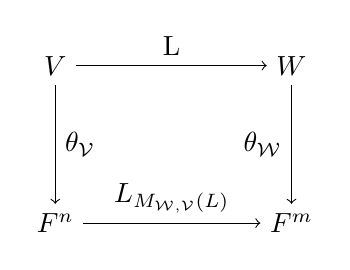
\begin{tikzpicture}
	\node (V) at (0,2) {$V$};
	\node (Fn) at (0,0) {$\mathbb{F}^n$};
	\node (W) at (3,2) {$W$};
	\node (Fm) at (3,0) {$\mathbb{F}^m$};

	\draw[->] (V) -- (Fn)  node[midway,right] {$\theta_\mathcal{V}$};
	\draw[->] (Fn) -- (Fm) node[midway,above] {$L_{M_{\mathcal{W},\mathcal{V}}(L)}$};
	\draw[->] (V) -- (W)   node[midway,above] {L};
	\draw[->] (W) -- (Fm)  node[midway,left] {$\theta_\mathcal{W}$};
\end{tikzpicture}

\end{center}

\section{Matrixrepræsentationen}
\begin{saetning}{4.2.1}
	Lad $L: \mathbb{F}^n \rightarrow \mathbb{F}^m$ være en lineær
	transformation.	

	Vi definerer $M(L) \in \mat_{m,n}(\mathbb{F})$ ved $M(L) = [L(\vec{e_1}), 
	\cdots, L(\vec{e_n})]$.
	Så er $L(\vec{x}) = M(L)\vec{x}$ for alle $\vec{x} \in \mathbb{F}^n$ og 
	$M(L)$ er den entydige matix med denne egenskab.
\end{saetning}

\begin{bevis}
	Lad $\vec{x} = \begin{bmatrix}x_1\\ \vdots \\ x_n\end{bmatrix} \in 
	\mathbb{F}^n$, så kan $x$ skrives som en lineær kombination: $\vec{x} = 
	x_1\vec{e_1} + \cdots + x_n\vec{e_n}$. Da må det gælde at:
	\begin{align*}	
		L(\vec{x}) &= L(x_1\vec{e_1} + \dotsb + x_n\vec{e_n}) \\
				   &= x_1L(\vec{e_1}) + \dotsb + x_nL(\vec{e_n}) \\
				   &= [L(\vec{e_1}), \dotsc, L(\vec{e_n})]
					\begin{bmatrix}
						x_1 \\
						\vdots \\
						x_n
					\end{bmatrix} \\
				   &= M(L)\vec{x}
	\end{align*}
	Entydighed: Hvis vi antager at $A \in \mat_{m,n}(\mathbb{F})$ 
	tilfredsstiller $L(\vec{x}) = A\vec{x}$ for alle $\vec{x} \in 
	\mathbb{F}^n$, så gælder dette specielt for $\vec{x} = \vec{e_i}$ hvor
	$i = 1, \dotsc, n$ at $L(\vec{e_i}) = A\vec{e_i} \Ra \{\text{i'te søjle i } 
	$A$\} = \{\text{i'te søjle i }$M(L)$\}$.
\end{bevis}

%
% Sætning 4.2.4 ([L] 4.2.2) side 67
% 

\begin{saetning}{4.2.4}
	Lad $V$, $W$ være $\mathbb{F}$-vektorrum og lad $\mathcal{V}=\{\vec{v}_1,
	\cdots,\vec{v}_n\}$, $\mathcal{W}=\{\vec{w}_1,\cdots,\vec{w}_n\}$ være
	ordnede baser for $V$, $W$. Lad $L \colon V \ra W$ være en lineær transformation.
	\[
		M_{\mathcal{W},\mathcal{V}} = [[L(\vec{v_1})]_\mathcal{W}, \cdots,
		[L(\vec{v_n})]_\mathcal{W}]
	\]
	Der gælder, at $[L(\vec{v})]_\mathcal{W} = M_{\mathcal{W},\mathcal{V}}
	[\vec{v}]_\mathcal{W}$ for alle $\vec{v} \in V$, samt at
	$M_{\mathcal{W},\mathcal{V}}$ er den entydige matrix med denne egenskab.
\end{saetning}

\begin{bevis}
	Lad $\vec{v} \in V$ hvor $\vec{v} = x_1 \vec{v_1} + \cdots + x_1 \vec{v_n}$
	og $\begin{bmatrix} x_1 \\ \vdots \\ x_n \end{bmatrix} =
	[\vec{v}]_\mathcal{V}$. Vi har
	\[
		L(\vv) = L(x_1 \vec{v_1} + \cdots + x_n \vec{v_n}) = x_1L(\vec{v_1}) + 
		\dotsc + x_nL(\vec{v_n})
	\]
	så
	\begin{align*}
		[L(\vv)]_\sW =& [x_1 L(\vec{v_1}) + \cdots + x_n L(\vec{v_n})]_\sW \\
			=& x_1 [L(\vec{v_1})]_\sW + \cdots + x_n [L(\vec{v_n})]_\sW \\
			=& \left[ [L(\vec{v_1})]_\sW, \cdots, [L(\vec{v_n})]_\sW
				\right] \begin{bmatrix}
					x_1 \\
					\vdots \\
					x_n
				\end{bmatrix} \\
			=& M_{\sV,\sW} [\vv]_\sV
	\end{align*}

	Hvis $A \in Mat_{m,n}(\mathbb{F})$ tilfredsstiller at
	\[
		[L(\vv_i)]_\sW = A[\vec{v_i}]_\sV = Ae_i = \{i \text{'te søjle i } A\}
	\]
	Så har $M_{\sV,\sW}(L)$ og $A$ de samme søjler og er derfor ens.
\end{bevis}

